\subsubsection{FAC}

\paragraph{Dendrograma de los clústeres obtenidos para FAC}

\begin{figure}[H]
    \centering
    
    \subfigure[\textit{HR}]{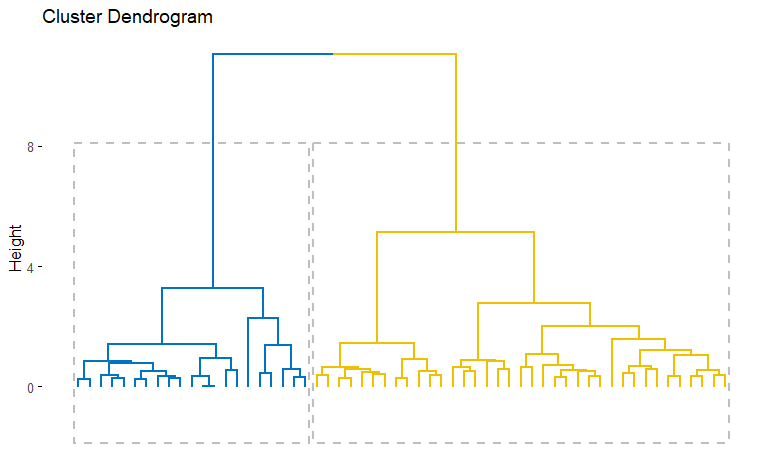
\includegraphics[width=0.45\textwidth]{img/01-1-acf.png}}
    \subfigure[\textit{HR\_scaled}]{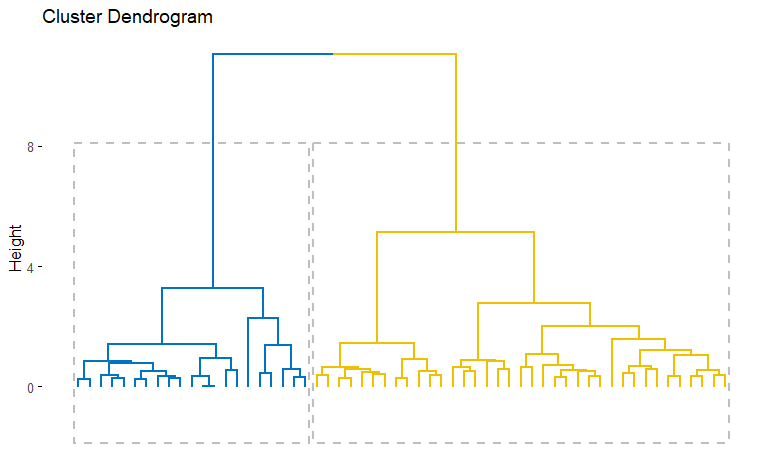
\includegraphics[width=0.45\textwidth]{img/02-1-acf.png}}
    \subfigure[\textit{HR\_quantile}]{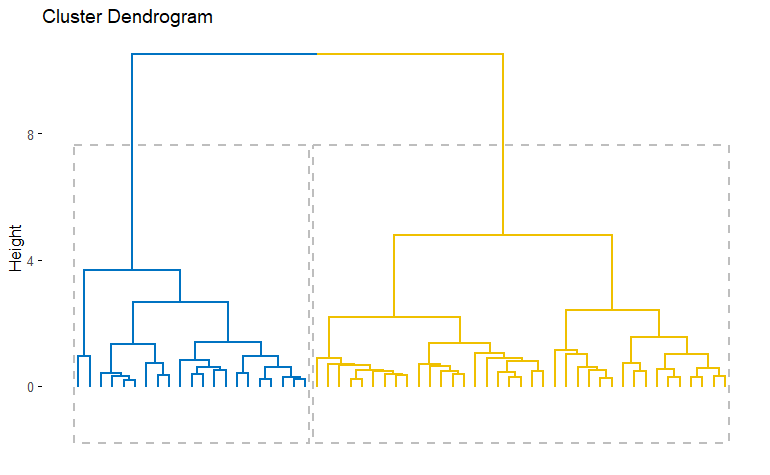
\includegraphics[width=0.5\textwidth]{img/03-1-acf.png}}
    \caption{Dendogramas usando FAC de \textit{HR}, \textit{HR\_scaled} y \textit{HR\_quantile}}
    \label{fig:acf_den_fc}
\end{figure}

\begin{figure}[ht]
    \centering
    \subfigure[\textit{SpO2}]{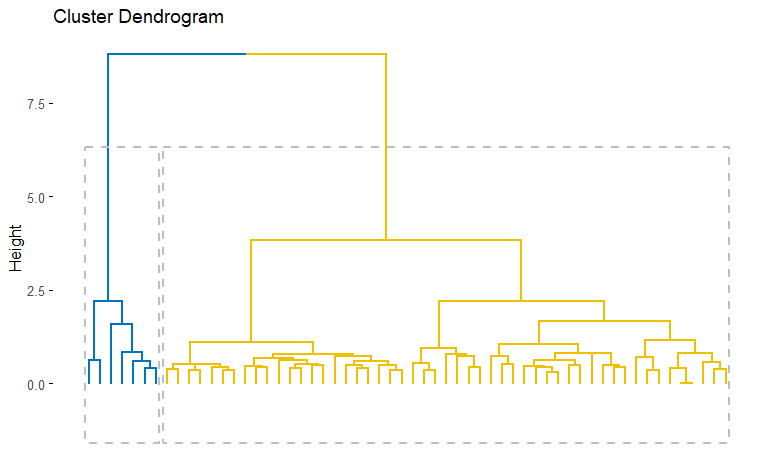
\includegraphics[width=0.5\textwidth]{img/04-1-acf.png}}\hfill
    \subfigure[\textit{SpO2\_scaled}]{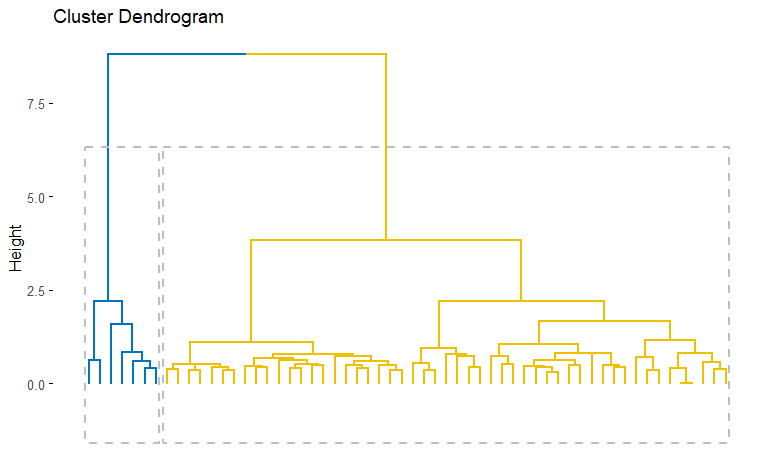
\includegraphics[width=0.5\textwidth]{img/05-1-acf.png}}
    \caption{Dendogramas usando FAC de \textit{SpO2} y \textit{SpO2\_scaled}}\label{fig:acf_den_spo2}
\end{figure}

\paragraph{Distribución de los clústeres obtenidos en función de las dos primeras componentes principales para FAC}

\begin{figure}[H]
    \centering
    \subfigure[\textit{HR}]{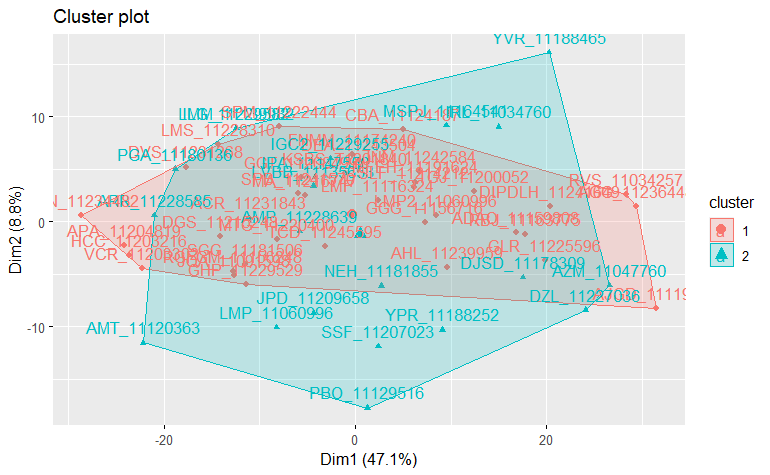
\includegraphics[width=0.45\textwidth]{img/01-2-acf.png}}
    \subfigure[\textit{HR\_scaled}]{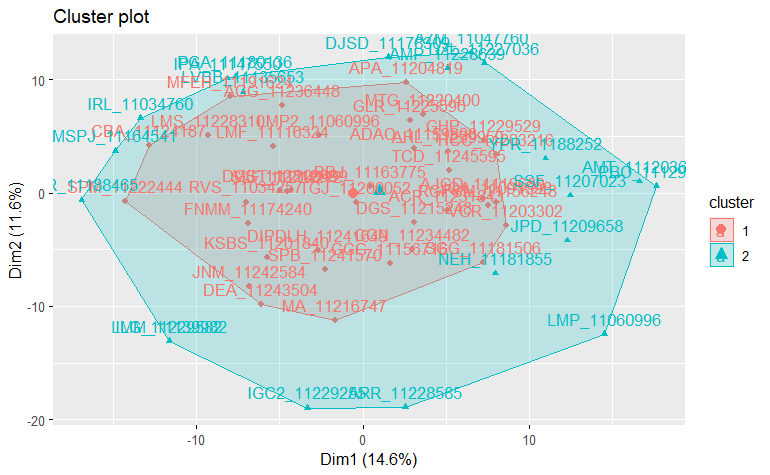
\includegraphics[width=0.45\textwidth]{img/02-2-acf.png}}
    \subfigure[\textit{HR\_quantile}]{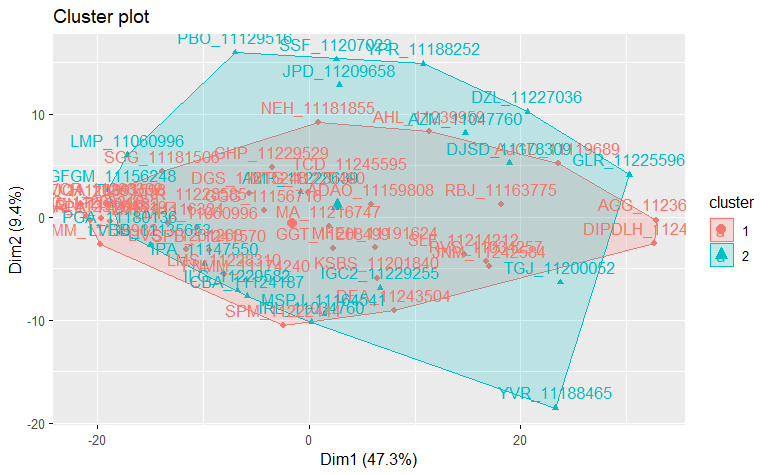
\includegraphics[width=0.5\textwidth]{img/03-2-acf.png}}
    \caption{Cluster Plot usando FAC de \textit{HR}, \textit{HR\_scaled} y \textit{HR\_quantile}}
    \label{fig:acf_pc_fc}
\end{figure}

\begin{figure}[H]
    \centering
    \subfigure[\textit{SpO2}]{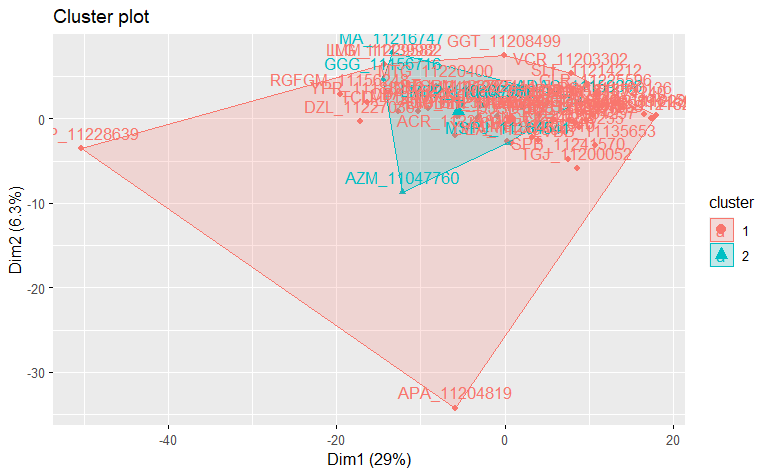
\includegraphics[width=0.5\textwidth]{img/04-2-acf.png}}\hfill
    \subfigure[\textit{SpO2\_scaled}]{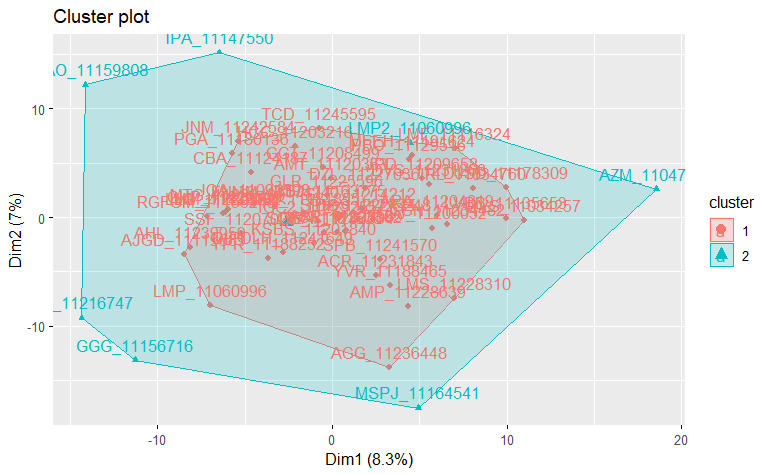
\includegraphics[width=0.5\textwidth]{img/05-2-acf.png}}
    \caption{Cluster Plot usando FAC de \textit{SpO2} y \textit{SpO2\_scaled}}\label{fig:acf_pc_spo2}
\end{figure}


\paragraph{Puntuación de Silhouette de los clústeres obtenidos para FAC}

\begin{figure}[H]
    \centering
    \subfigure[\textit{HR}]{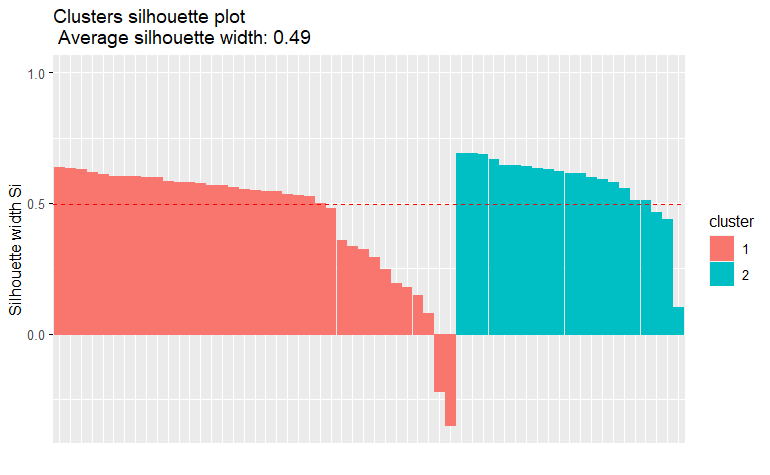
\includegraphics[width=0.45\textwidth]{img/01-3-acf.png}}
    \subfigure[\textit{HR\_scaled}]{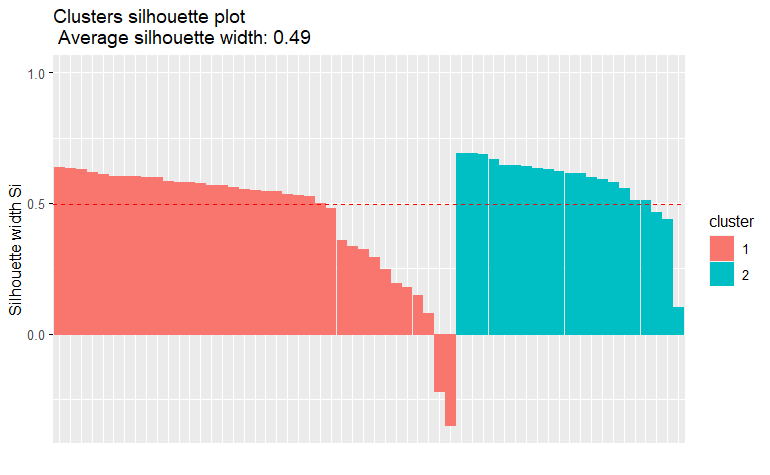
\includegraphics[width=0.45\textwidth]{img/02-3-acf.png}}
    \subfigure[\textit{HR\_quantile}]{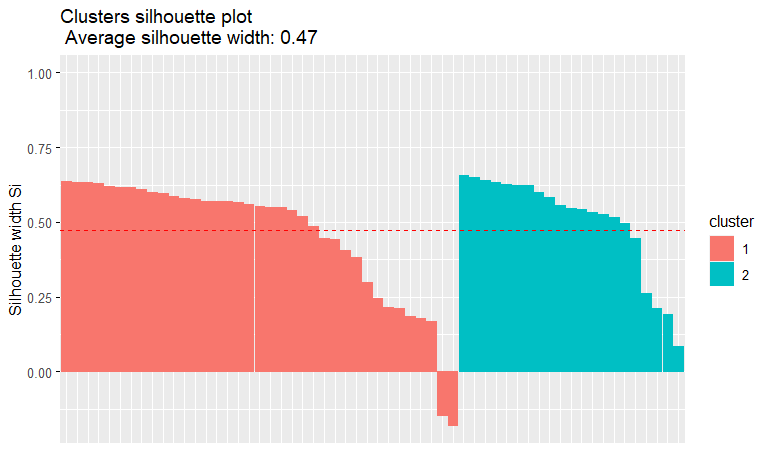
\includegraphics[width=0.5\textwidth]{img/03-3-acf.png}}
    \caption{Silhouette Plot usando FAC de \textit{HR}, \textit{HR\_scaled} y \textit{HR\_quantile}}\label{fig:acf_si_fc}
\end{figure}

\begin{figure}[ht]
    \centering
    \subfigure[\textit{SpO2}]{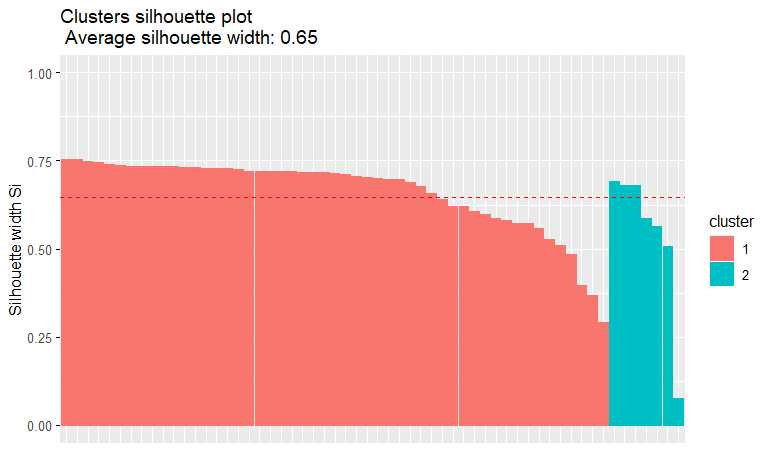
\includegraphics[width=0.5\textwidth]{img/04-3-acf.png}}\hfill
    \subfigure[\textit{SpO2\_scaled}]{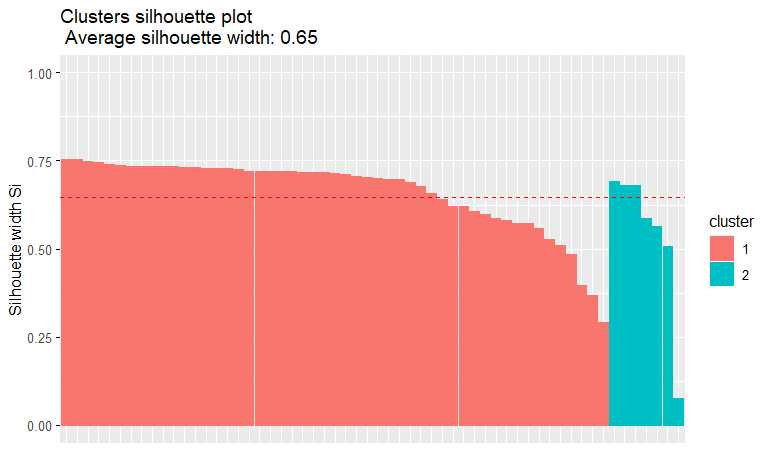
\includegraphics[width=0.5\textwidth]{img/05-3-acf.png}}
    \caption{Silhouette Plot usando FAC de \textit{SpO2} y \textit{SpO2\_scaled}}\label{fig:acf_si_spo2}
\end{figure}

\paragraph{Dendograma dividido en dos clústeres según los pacientes que han experimentado OAF para FAC}

\begin{figure}[H]
    \centering
    \subfigure[\textit{HR}]{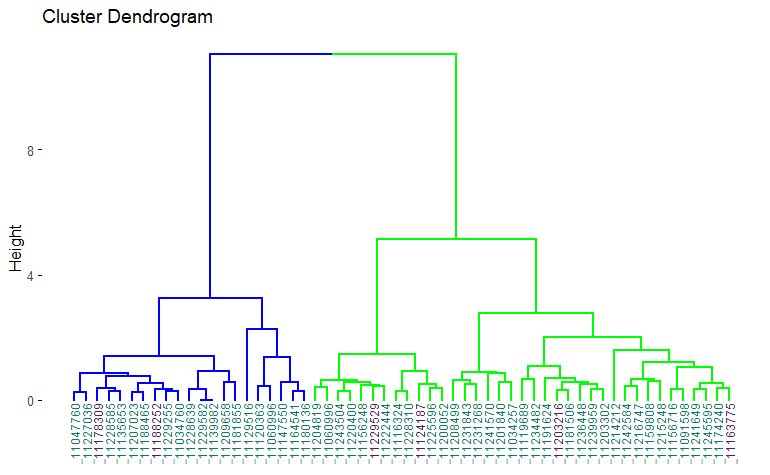
\includegraphics[width=0.45\textwidth]{img/01-4-acf.png}}
    \subfigure[\textit{HR\_scaled}]{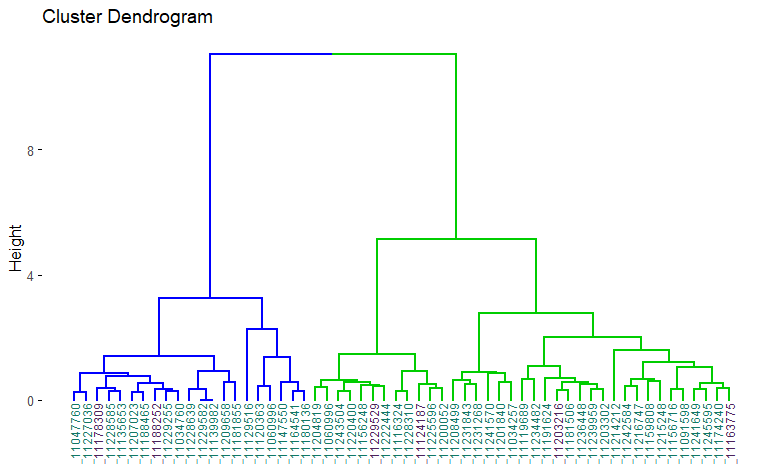
\includegraphics[width=0.45\textwidth]{img/02-4-acf.png}}
    \subfigure[\textit{HR\_quantile}]{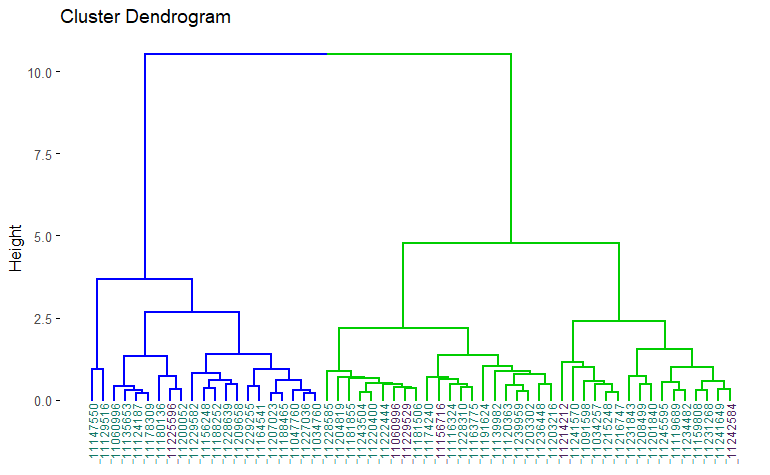
\includegraphics[width=0.5\textwidth]{img/03-4-acf.png}}
    \caption{Dendograma Plot k = 2 usando FAC de \textit{HR}, \textit{HR\_scaled} y \textit{HR\_quantile}}\label{fig:acf_ctg_fc}
\end{figure}

\begin{figure}[ht]
    \centering
    \subfigure[\textit{SpO2}]{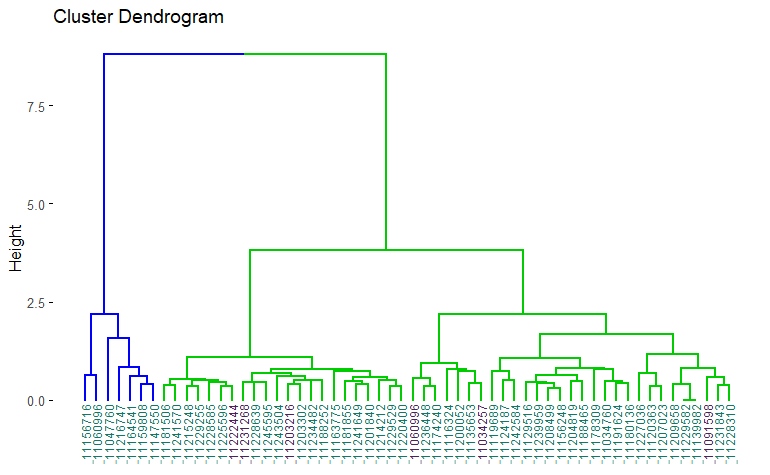
\includegraphics[width=0.5\textwidth]{img/04-4-acf.png}}\hfill
    \subfigure[\textit{SpO2\_scaled}]{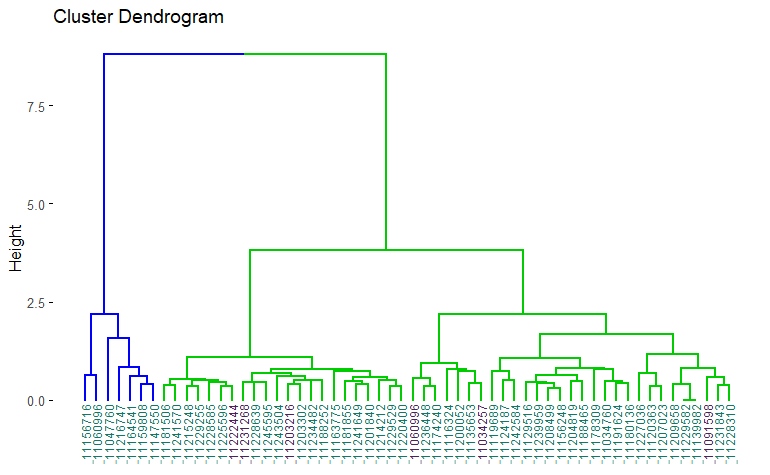
\includegraphics[width=0.5\textwidth]{img/05-4-acf.png}}
    \caption{Dendograma Plot k = 2 usando FAC de \textit{SpO2} y \textit{SpO2\_scaled}}\label{fig:acf_ctg_spo2}
\end{figure}

\paragraph{Clasificación mediente Random Forest de los clústeres generados con los datos de {\color{blue}Periodograma} según las variables \textit{Cuantitativas} y \textit{Cualitativas} de la Tabla~\ref{tabla:variables_estudio_final} para FAC}

\begin{figure}[H]
    \centering
    \begin{lstlisting}[frame=single, basicstyle=\small\ttfamily]
        randomForest(formula = CLUSTER ~ ., data = newSMOTE_ACF) 
               Type of random forest: classification
                     Number of trees: 500
No. of variables tried at each split: 5

        OOB estimate of  error rate: 48.28%
Confusion matrix:
   1  2 class.error
1 26 11   0.2972973
2 17  4   0.8095238
    \end{lstlisting}
    \caption{Resultado de Random Forest usando FAC para \textit{HR} utilizando variables \textit{Cuantitativas} y \textit{Cualitativas} de la Tabla~\ref{tabla:variables_estudio_final} y clasificación de clusters k = 2}\label{fig:random_forest_acf_result_1}
\end{figure}
\begin{figure}[H]
    \centering
    \begin{lstlisting}[frame=single, basicstyle=\small\ttfamily]
        randomForest(formula = CLUSTER ~ ., data = newSMOTE_ACF) 
               Type of random forest: classification
                     Number of trees: 500
No. of variables tried at each split: 5

        OOB estimate of  error rate: 48.28%
Confusion matrix:
   1  2 class.error
1 26 11   0.2972973
2 17  4   0.8095238
    \end{lstlisting}
    \caption{Resultado de Random Forest usando FAC para \textit{HR\_scaled} utilizando variables \textit{Cuantitativas} y \textit{Cualitativas} de la Tabla~\ref{tabla:variables_estudio_final} y clasificación de clusters k = 2}
    \label{fig:random_forest_acf_result_2}
\end{figure}

\begin{figure}[H]
    \centering
    \begin{lstlisting}[frame=single, basicstyle=\small\ttfamily]
        randomForest(formula = CLUSTER ~ ., data = newMWMOTE_ACF) 
               Type of random forest: classification
                     Number of trees: 500
No. of variables tried at each split: 5

        OOB estimate of  error rate: 32.76%
Confusion matrix:
   1 2 class.error
1 30 7   0.1891892
2 12 9   0.5714286
    \end{lstlisting}
    \caption{Resultado de Random Forest usando FAC para \textit{HR\_quantile} utilizando variables \textit{Cuantitativas} y \textit{Cualitativas} de la Tabla~\ref{tabla:variables_estudio_final} y clasificación de clusters k = 2}
    \label{fig:random_forest_acf_result_3}
\end{figure}

\begin{figure}[H]
    \centering
    \begin{lstlisting}[frame=single, basicstyle=\small\ttfamily]
        randomForest(formula = CLUSTER ~ ., data = newSMOTE_ACF) 
               Type of random forest: classification
                     Number of trees: 500
No. of variables tried at each split: 5

        OOB estimate of  error rate: 5.26%
Confusion matrix:
   1  2 class.error
1 49  2  0.03921569
2  3 41  0.06818182
    \end{lstlisting}
    \caption{Resultado de Random Forest usando FAC para \textit{SpO2} utilizando variables \textit{Cuantitativas} y \textit{Cualitativas} de la Tabla~\ref{tabla:variables_estudio_final} y clasificación de clusters k = 2}\label{fig:random_forest_acf_result_4}
\end{figure}
\begin{figure}[H]
    \centering
    \begin{lstlisting}[frame=single, basicstyle=\small\ttfamily]
        randomForest(formula = CLUSTER ~ ., data = newSMOTE_ACF) 
               Type of random forest: classification
                     Number of trees: 500
No. of variables tried at each split: 5

        OOB estimate of  error rate: 5.26%
Confusion matrix:
   1  2 class.error
1 49  2  0.03921569
2  3 41  0.06818182
    \end{lstlisting}
    \caption{Resultado de Random Forest usando FAC para \textit{SpO2\_scaled} utilizando variables \textit{Cuantitativas} y \textit{Cualitativas} de la Tabla~\ref{tabla:variables_estudio_final} y clasificación de clusters k = 2}
    \label{fig:random_forest_acf_result_5}
\end{figure}

\paragraph{Mean Decrease Accuracy de las 5 primeras variables descriptivas utilizadas en Random Forest para FAC}

\begin{table}[H]
    \centering
    \begin{tabular}{lr}
        \toprule
        \textbf{Variable} & \textbf{Mean Decrease Accuracy} \\
        \midrule
        EDAD & 2.6328715 \\
        SCORE\_WOOD\_DOWNES\_INGRESO & 2.5338316 \\
        PESO & 2.3967813 \\
        SCORE\_CRUCES\_INGRESO & 2.3630299 \\
        FR\_0\_8h & 1.7007907 \\
        \bottomrule
    \end{tabular}
    \caption{Mean Decrease Accuracy usando FAC \textit{HR}}
\end{table}

\begin{table}[H]
    \centering
    \begin{tabular}{lr}
        \toprule
        \textbf{Variable} & \textbf{Mean Decrease Accuracy} \\
        \midrule
        EDAD & 2.6328715 \\
        SCORE\_WOOD\_DOWNES\_INGRESO & 2.5338316 \\
        PESO & 2.3967813 \\
        SCORE\_CRUCES\_INGRESO & 2.3630299 \\
        FR\_0\_8h & 1.7007907 \\
        \bottomrule
    \end{tabular}
    \caption{Mean Decrease Accuracy usando FAC \textit{HR\_scaled}}
\end{table}

\begin{table}[H]
    \centering
    \begin{tabular}{lr}
        \toprule
        \textbf{Variable} & \textbf{Mean Decrease Accuracy} \\
        \midrule
        SCORE\_WOOD\_DOWNES\_INGRESO & 3.1336476 \\
        PESO & 3.1080877 \\
        EDAD & 2.5533093 \\
        SCORE\_CRUCES\_INGRESO & 2.3892629 \\
        FR\_0\_8h & 1.7130177 \\
        \bottomrule
    \end{tabular}
    \caption{Mean Decrease Accuracy usando FAC \textit{HR\_quantile}} 
\end{table}

\begin{table}[H]
    \centering
    \begin{tabular}{lr}
        \toprule
        \textbf{Variable} & \textbf{Mean Decrease Accuracy} \\
        \midrule
        SCORE\_CRUCES\_INGRESO & 6.6714244 \\
        SAPI\_0\_8h & 6.2990402 \\
        SCORE\_WOOD\_DOWNES\_INGRESO & 5.7922765 \\
        ENFERMEDAD\_BASE & 4.3830928 \\
        EDAD & 2.9415274 \\
        \bottomrule
    \end{tabular}
    \caption{Mean Decrease Accuracy usando FAC \textit{SpO2}}
\end{table}

\begin{table}[H]
    \centering
    \begin{tabular}{lr}
        \toprule
        \textbf{Variable} & \textbf{Mean Decrease Accuracy} \\
        \midrule
        SAPI\_0\_8h & 7.3979738 \\
        SCORE\_CRUCES\_INGRESO & 6.7882670 \\
        SCORE\_WOOD\_DOWNES\_INGRESO & 5.2945505 \\
        ENFERMEDAD\_BASE & 3.1331112 \\
        DIAS\_GN & 3.0845580 \\
        \bottomrule
    \end{tabular}
    \caption{Mean Decrease Accuracy usando FAC \textit{SpO2\_scaled}}
\end{table}


\paragraph{Clasificación {\color{blue}mediante} Random Forest de los clústeres según FAC utilizada para {\color{blue}generar} los mismos} 

\begin{figure}[H]
    \centering
    \begin{lstlisting}[frame=single, basicstyle=\small\ttfamily]
        randomForest(formula = CLUSTER ~ ., data = data_frame_merge_ACF) 
               Type of random forest: classification
                     Number of trees: 500
No. of variables tried at each split: 7

        OOB estimate of  error rate: 1.72%
Confusion matrix:
   1  2 class.error
1 37  0  0.00000000
2  1 20  0.04761905
    \end{lstlisting}
    \caption{Resultado de Random Forest usando FAC para \textit{HR} utilizando FAC y clasificación de clusters k = 2}\label{fig:random_forest_acf_result_RF_1}
\end{figure}
\begin{figure}[H]
    \centering
    \begin{lstlisting}[frame=single, basicstyle=\small\ttfamily]
        randomForest(formula = CLUSTER ~ ., data = data_frame_merge_ACF) 
               Type of random forest: classification
                     Number of trees: 500
No. of variables tried at each split: 7

        OOB estimate of  error rate: 1.72%
Confusion matrix:
   1  2 class.error
1 37  0  0.00000000
2  1 20  0.04761905
    \end{lstlisting}
    \caption{Resultado de Random Forest usando FAC para \textit{HR\_scaled} utilizando FAC y clasificación de clusters k = 2}
    \label{fig:random_forest_acf_result_RF_2}
\end{figure}

\begin{figure}[H]
    \centering
    \begin{lstlisting}[frame=single, basicstyle=\small\ttfamily]
        randomForest(formula = CLUSTER ~ ., data = data_frame_merge_ACF) 
               Type of random forest: classification
                     Number of trees: 500
No. of variables tried at each split: 7

        OOB estimate of  error rate: 3.45%
Confusion matrix:
   1  2 class.error
1 36  1  0.02702703
2  1 20  0.04761905
    \end{lstlisting}
    \caption{Resultado de Random Forest usando FAC para \textit{HR\_quantile} utilizando FAC y clasificación de clusters k = 2}
    \label{fig:random_forest_acf_result_RF_3}
\end{figure}

\begin{figure}[H]
    \centering
    \begin{lstlisting}[frame=single, basicstyle=\small\ttfamily]
        randomForest(formula = CLUSTER ~ ., data = data_frame_merge_ACF) 
               Type of random forest: classification
                     Number of trees: 500
No. of variables tried at each split: 7

        OOB estimate of  error rate: 1.72%
Confusion matrix:
   1 2 class.error
1 51 0   0.0000000
2  1 6   0.1428571
    \end{lstlisting}
    \caption{Resultado de Random Forest usando FAC para \textit{SpO2} utilizando FAC y clasificación de clusters k = 2}\label{fig:random_forest_acf_result_RF_4}
\end{figure}
\begin{figure}[H]
    \centering
    \begin{lstlisting}[frame=single, basicstyle=\small\ttfamily]
        randomForest(formula = CLUSTER ~ ., data = data_frame_merge_ACF) 
               Type of random forest: classification
                     Number of trees: 500
No. of variables tried at each split: 7

        OOB estimate of  error rate: 1.72%
Confusion matrix:
   1 2 class.error
1 51 0   0.0000000
2  1 6   0.1428571
    \end{lstlisting}
    \caption{Resultado de Random Forest usando FAC para \textit{SpO2\_scaled} utilizando FAC y clasificación de clusters k = 2}
    \label{fig:random_forest_acf_result_RF_5}
\end{figure}

\paragraph{Distribución de la Importancia de FAC}

\begin{figure}[H]
    \centering
    \subfigure[\textit{HR}]{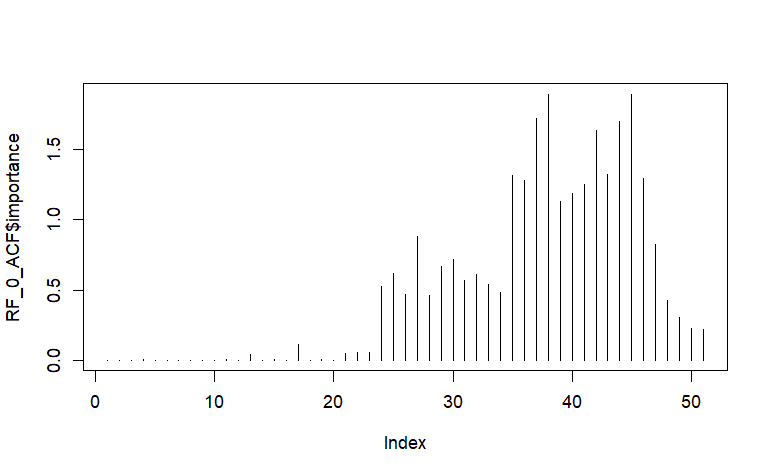
\includegraphics[width=0.45\textwidth]{img/01-5-acf.png}}
    \subfigure[\textit{HR\_scaled}]{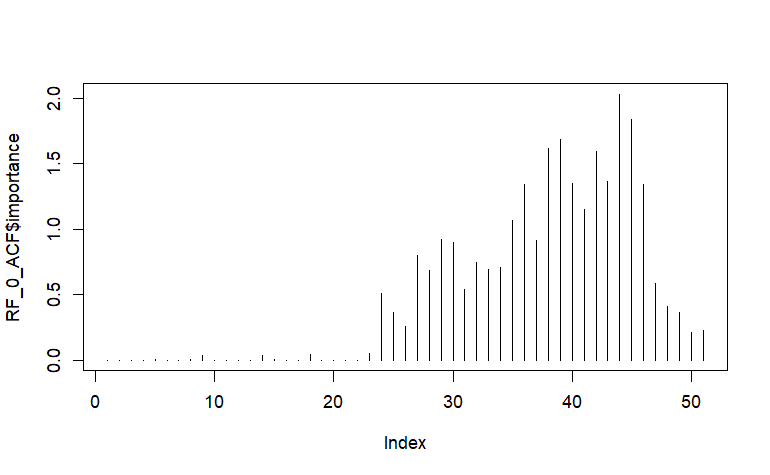
\includegraphics[width=0.45\textwidth]{img/02-5-acf.png}}
    \subfigure[\textit{HR\_quantile}]{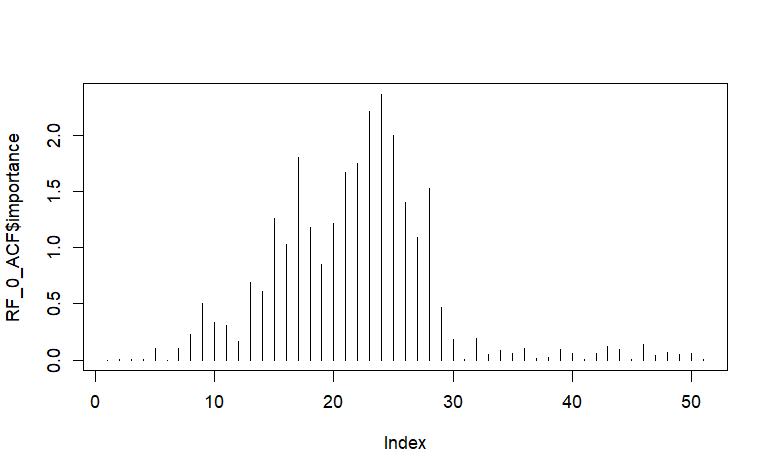
\includegraphics[width=0.5\textwidth]{img/03-5-acf.png}}
    \caption{Importancia FAC de \textit{HR}, \textit{HR\_scaled} y \textit{HR\_quantile}}\label{fig:acf_imp_fc}
\end{figure}

\begin{figure}[ht]
    \centering
    \subfigure[\textit{SpO2}]{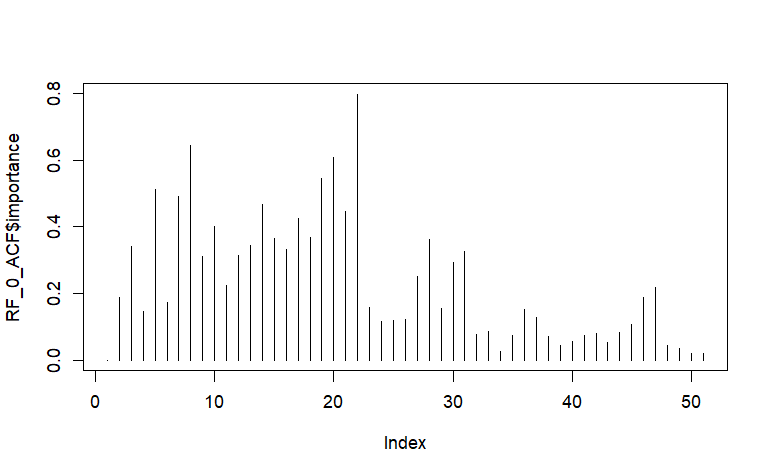
\includegraphics[width=0.5\textwidth]{img/04-5-acf.png}}\hfill
    \subfigure[\textit{SpO2\_scaled}]{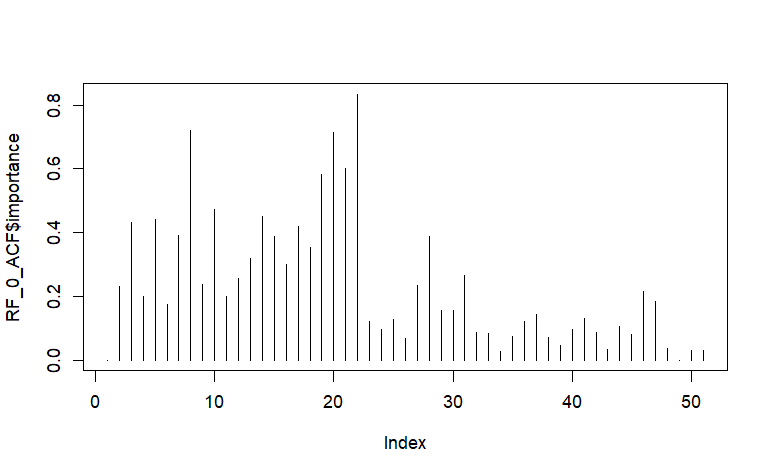
\includegraphics[width=0.5\textwidth]{img/05-5-acf.png}}
    \caption{Importancia FAC de \textit{SpO2} y \textit{SpO2\_scaled}}\label{fig:acf_imp_spo2}
\end{figure}


\paragraph{Media de los valores de FAC en función de los clusters generados $k = 2$}

\begin{figure}[H]
    \centering
    \subfigure[\textit{HR}]{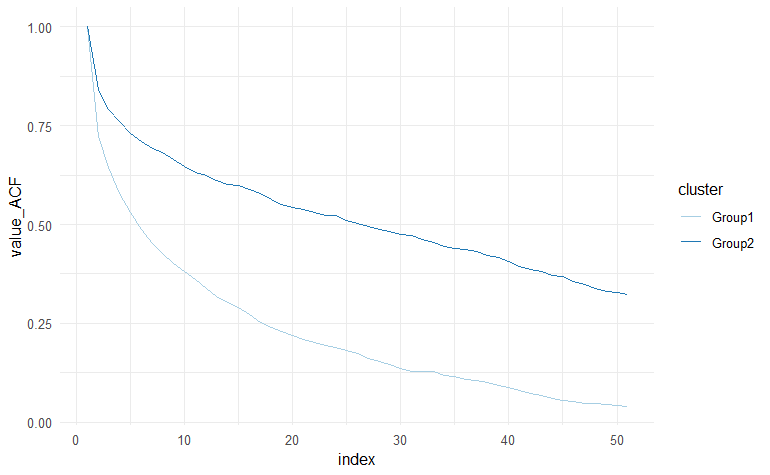
\includegraphics[width=0.45\textwidth]{img/01-6-acf.png}}
    \subfigure[\textit{HR\_scaled}]{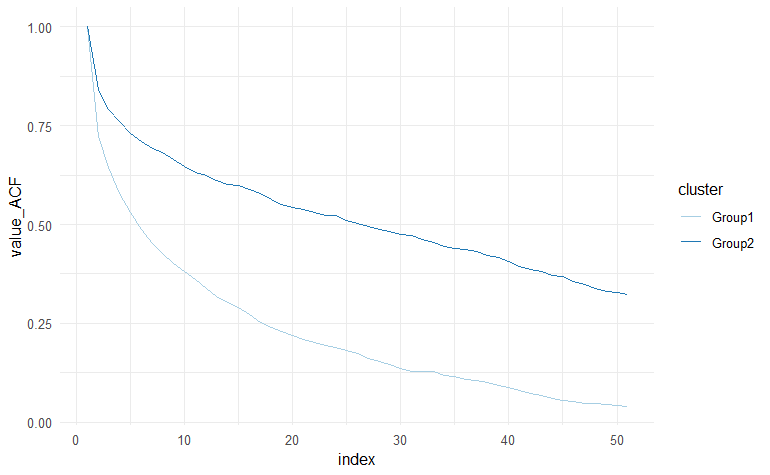
\includegraphics[width=0.45\textwidth]{img/02-6-acf.png}}
    \subfigure[\textit{HR\_quantile}]{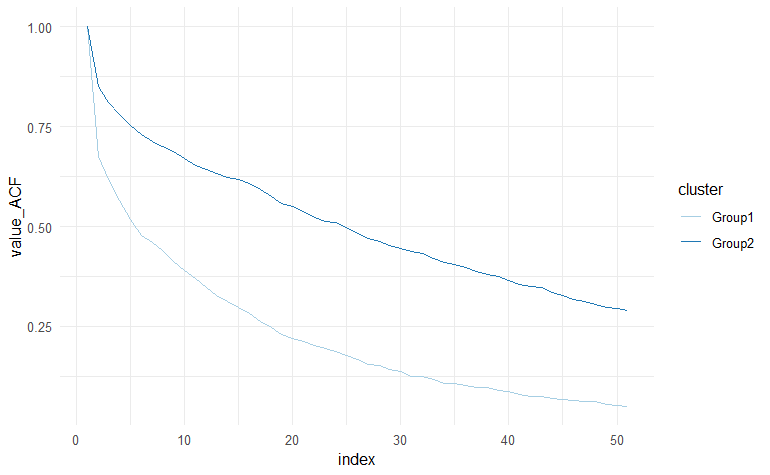
\includegraphics[width=0.5\textwidth]{img/03-6-acf.png}}
    \caption{Valores de FAC por cluster k = 2 de \textit{HR}, \textit{HR\_scaled} y \textit{HR\_quantile}}\label{fig:acf_cls_fc}
\end{figure}

\begin{figure}[ht]
    \centering
    \subfigure[\textit{SpO2}]{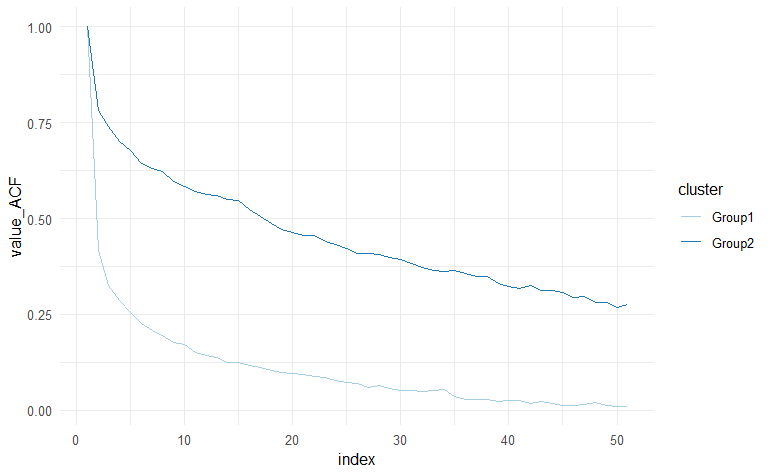
\includegraphics[width=0.5\textwidth]{img/04-6-acf.png}}\hfill
    \subfigure[\textit{SpO2\_scaled}]{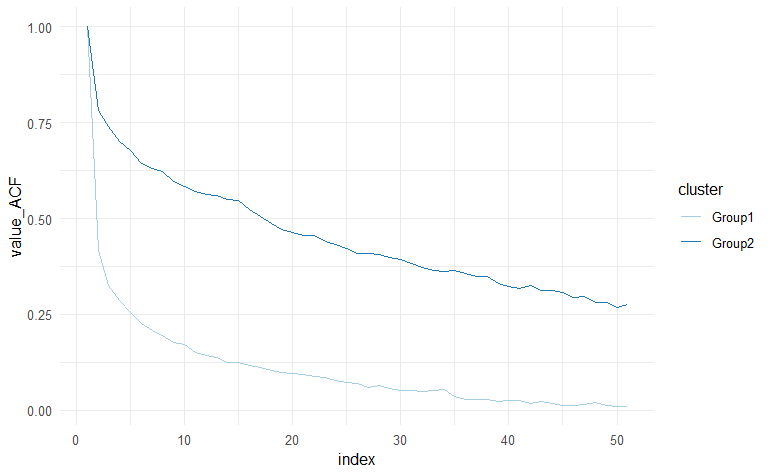
\includegraphics[width=0.5\textwidth]{img/05-6-acf.png}}
    \caption{Valores de FAC por cluster k = 2 de \textit{SpO2} y \textit{SpO2\_scaled}}\label{fig:acf_cls_spo2}
\end{figure}

